\documentclass[a4paper,11pt]{article}
\renewcommand{\baselinestretch}{1.5} %% Change the baseline stretch to 1.5 
\usepackage{geometry}
 \geometry{
 a4paper,
 total={170mm,257mm},
 left=20mm,
 top=20mm,
 }

 \usepackage{wrapfig}
 \usepackage[utf8x]{inputenc}
 \usepackage{amsmath}
\usepackage{amssymb}
 \usepackage{siunitx}
 \usepackage{multirow}
\usepackage{colortbl}
 \usepackage{hhline}

 \usepackage{lipsum}  %%% Lorem ipsum

\setlength{\headheight}{30.0pt}
\setlength{\footskip}{20pt}

%%%%%%%%%%%%%%%%TABLE
\setlength{\arrayrulewidth}{0.5mm}
\setlength{\tabcolsep}{18pt}
\renewcommand{\arraystretch}{1.5}
%%%%%%%%%%%%

\usepackage{hyperref}
\hypersetup{
    colorlinks=True,
    linkcolor={blue!20!black},
    filecolor=magenta,      
    urlcolor=cyan,
}



 \usepackage[export]{adjustbox}
\usepackage[english]{babel}
\usepackage{fancyhdr}
\usepackage{multicol}

\pagestyle{fancy}
\fancyhf{}
\rhead{\textit{Pul074BEX004}}
\lhead{\textit{Amrit Prasad Phuyal}}
\rfoot{\thepage}


\usepackage{mathpazo} % Palatino font
\usepackage{graphicx}
\usepackage{float}
\usepackage{xcolor}
\usepackage{color}

%%%% Anser environment use %%%% Anser environment use %%%% Anser environment use \input{./AnsENV.tex}
%% use \begin{A... {**** argument***}
\RequirePackage{scrextend}

\newenvironment{A}[1]{\textit{Answer:}{\begin{addmargin}[2em]{2em}{#1}\end{addmargin} 
  }}

% just leave some space   
%% use \begin{A... {**** argument***}
\RequirePackage{scrextend}

\newenvironment{A}[1]{\textit{Answer:}{\begin{addmargin}[2em]{2em}{#1}\end{addmargin} 
  }}

% just leave some space   
%% use \begin{A... {**** argument***}
\RequirePackage{scrextend}

\newenvironment{A}[1]{\textit{Answer:}{\begin{addmargin}[2em]{2em}{#1}\end{addmargin} 
  }}

% just leave some space    %% Answer environment 

%%% Question Environment%%%  use 
%%% Question Environment%%%  use 
%%% Question Environment%%%  use \input{./QueENV.tex}   to include
%% Use \begin{Q}....\end{Q}

\newcounter{QC}
\setcounter{QC}{1}
\newenvironment{Q}[1]{
    \section{Question -\arabic{QC}} \stepcounter{QC}{\large\textbf{#1}}
}

%%% Question Environment%%%

   to include
%% Use \begin{Q}....\end{Q}

\newcounter{QC}
\setcounter{QC}{1}
\newenvironment{Q}[1]{
    \section{Question -\arabic{QC}} \stepcounter{QC}{\large\textbf{#1}}
}

%%% Question Environment%%%

   to include
%% Use \begin{Q}....\end{Q}

\newcounter{QC}
\setcounter{QC}{1}
\newenvironment{Q}[1]{
    \section{Question -\arabic{QC}} \stepcounter{QC}{\large\textbf{#1}}
}

%%% Question Environment%%%

 %% Question Environment 
%%%%%% include  Titles.%%%% use \input{./CP}%%%
%%%use """"""""    \CP{}{}{}{}   """" %%%% and 4 argument to craete Title page 
%%%%%%%%%%%%%%%%%%%%%%%%%%%%%%%%%%%%%%%%%%%%%%%%%%%%%%%%%%%%%%%%%
%%%argument number
%% 1=major header ## Course name 
%% 2=minor4 heading ## lab/assignmet no
%% 3=Title  ## Assignment or Lab title
%% 4=submitted to::## input receiver Name"
%%%%%%%%%%%%%%%%%%%%%%%%%%%%%%%%%%%%%%%%%%%%%%%%%%%%%%%%%%%%%%%%%


\usepackage{mathpazo} % Palatino font
\usepackage{graphicx}
\usepackage{float}

%%% format and command for lab ans c and assembly

\newcommand{\HRule}{\rule{\linewidth}{0.4mm}} % Defines a new command for horizontal lines, change thickness here



%----------------------------------------------------------------------------------------
%	TITLE PAGE
%----------------------------------------------------------------------------------------


\newcommand{\CP}[4]{ \begin{titlepage} % Suppresses displaying the page number on the title page and the subsequent page counts as page 1
		%%%%  univerdity logo%%
		\begin{figure}[H]
			\centering
			
\includegraphics[scale=0.13]{tulogo.jpg}
		\end{figure}
		%%% end university logo

		\center % Centre everything on the page

		%------------------------------------------------
		%	Headings
		%------------------------------------------------

		\textsc{\huge Institute of Engineering \\ Central Campus,Pulchowk}\\[1.5cm] % Main heading such as the name of your university/college

		\textsc{\Large #1}\\[0.5cm] % Major heading such as course name

		\textsc{\large #2}\\[0.5cm] % Minor heading such as assignment no./ lab no.

		%------------------------------------------------
		%	Title
		%------------------------------------------------

		\HRule\\[0.4cm]

		{\Huge\bfseries #3}\\[0.4cm] % Title of your document

		\HRule\\[1.5cm]

		%------------------------------------------------
		%	Author(s)
		%------------------------------------------------
		\vfill\vfill
		\begin{minipage}{0.4\textwidth}
			\begin{flushleft}
				\large{
				\textbf{Submitted BY:}\\
				{\normalsize AMRIT PRASAD PHUYAL}\\ % NAME
				{\normalsize Roll: PULL074BEX004}} % Roll
			\end{flushleft}
		\end{minipage}
		~
		\begin{minipage}{0.4\textwidth}
			\begin{flushright}
				\large
				\textbf{Submitted To:}\\
				{ \normalsize{#4}\\ }% recepent's  Name 
				{\normalsize Department of Electronics and Computer Engineering}
			\end{flushright}
		\end{minipage}

		%------------------------------------------------
		%	Date
		%------------------------------------------------

		\vfill\vfill\vfill % Position the date 3/4 down the remaining page

		{\large\today} % Date, change the \today to a set date if you want to be precise

		\vfill % Push the date up 1/4 of the remaining page

	\end{titlepage}
} %%% cover page


\usepackage{tikz}
\usepackage{circuitikz}
\newcommand\ddfrac[2]{\frac{\displaystyle #1}{\displaystyle #2}} 


\def\raa {R_{A}}
\def\rbb {R_{B}}
\def\vaa {V_A}
\def\vbb {V_B}
\def\va{V_1}
\def\vb{V_2}
\def\ra {R_1}
\def\rb {R_2}
\def\rc {R_3}
\def\rd {R_4}
\def\re {R_5}
\def\rf {R_6}
\def\ca {C_1}
\def\cb {C_2}

\def\Res #1{
    \SI{#1}{\ohm}
}

\newcommand{\figquestion}{
    \begin{circuitikz}
        \draw
        (0,0) to[R,l= \footnotesize$R_1\text{ = }1\text{ }\Omega$] (2,0) to [L,l=\footnotesize$L_1\text{ = }0.7654\text{ H}$] (4,0) to [C, *-*, l_=\footnotesize$C_1\text{ = }1.848 \text{ F}$] (4,-4)
        (4,0) to [L,l=\footnotesize$L_2\text{ = }1.848\text{ H}$] (8,0) to [C, *-*, l_=\footnotesize$C_2\text{ = }0.7654 \text{ F}$] (8,-4)
        (8,0) to [short] (12,0)
        (0,0) to [esource,v_=\footnotesize$V_1$] (0,-4)
        (0,-4) to [short] (12,-4) to[R, l=\footnotesize$R_2\text{ = }1\Omega$, v<=\footnotesize$V_2$] (12,0)
        ;
    \end{circuitikz}
}


\newcommand{\figfdnr}{
    \begin{circuitikz}
        \draw
        (0,0) to[C,l= \footnotesize$Z'_{R\textsubscript{$1$}}\text{ = }1\text{ F}$] (2,0) to [R,l=\footnotesize$Z'_{L\textsubscript{$1$}}\text{ = }0.7654\text{ }\Omega$] (4,0)  to [R,l=\footnotesize$Z'_{L\textsubscript{$2$}}\text{ = }1.848\text{ }\Omega$] (8,0) to [short] (12,0)
        (0,0) to [esource,v_=\footnotesize$V_1$] (0,-4)
        (0,-4) to [short] (12,-4) to[C, l=\footnotesize$Z'_{R\textsubscript{$2$}}\text{ = }1\text{ F}$, v<=\footnotesize$V_2$] (12,0)
        (4,0) to [short,*-] (4,-1.6)
        (4,-2.2) to [short,-*] (4,-4)
        (3.7,-2) node [left] {\footnotesize$Z'_{C\textsubscript{$1$}}\text{ = }1.848$}
        (8,0) to [short,*-] (8,-1.6)
        (8,-2.2) to [short,-*] (8,-4)
        (7.7,-2) node [left] {\footnotesize$Z'_{C\textsubscript{$2$}}\text{ = }0.7654$}
        ;
        \draw [thick] (3.7,-1.6)-- (4.3,-1.6);
        \draw [thick] (3.7,-1.8)-- (4.3,-1.8);
        \draw [thick] (3.7,-2)-- (4.3,-2);
        \draw [thick] (3.7,-2.2)-- (4.3,-2.2);

        \draw [thick] (7.7,-1.6)-- (8.3,-1.6);
        \draw [thick] (7.7,-1.8)-- (8.3,-1.8);
        \draw [thick] (7.7,-2)-- (8.3,-2);
        \draw [thick] (7.7,-2.2)-- (8.3,-2.2);

    \end{circuitikz}
}


\newcommand{\fighp}{
    \begin{circuitikz}
        \draw
        (0,0) to[R,l= \footnotesize$Z'_{R\textsubscript{$1$}}\text{ = }1\text{ }\Omega$] (2,0) to [C,l=\footnotesize$Z'_{L\textsubscript{$1$}}\text{ = }1.3065\text{ F}$] (4,0) to [L,l_=\footnotesize$Z'_{C\textsubscript{$1$}}\text{ = }0.5411\text{ H}$, *-*] (4,-4) (4,0) to [C,l=\footnotesize$Z'_{L\textsubscript{$2$}}\text{ = }0.5411\text{ F}$] (8,0) to [L,l_=\footnotesize$Z'_{C\textsubscript{$2$}}\text{ = }1.3065\text{ H}$, *-*] (8,-4)
        (8,0) to [short] (12,0)
        (0,0) to [esource,v_=\footnotesize$V_1$] (0,-4)
        (0,-4) to [short] (12,-4) to[R, l=\footnotesize$Z'_{R\textsubscript{$2$}}\text{ = }1\text{ }\Omega$, v<=\footnotesize$V_2$] (12,0)
        ;
    \end{circuitikz}
}


\newcommand{\figleap}{
    \begin{circuitikz}
        \draw
        (0,0) to[generic,l= \footnotesize$Z_1$,i_=\footnotesize$I_1$] (4,0) to [generic, *-*, l_=\footnotesize$Z_2$] (4,-4)
        (4,0) node (v3) [anchor=south] {\footnotesize$V_3$} to [generic,l=\footnotesize$Z_3$,i_=\footnotesize$I_2$] (8,0) (8,-4) to [generic, l=\footnotesize$Z_4$,*-*] (8,0) node (v4) [anchor=south] {\footnotesize$V_4$} to [short,-o] (9,0)
        (8,-4) to [short,-o] (9,-4)
        (0,0) to [esource,v_=\footnotesize$V_1$] (0,-4)
        (9,0) to [open,v^=\footnotesize$V_2$] (9,-4)
        (0,-4) to [short] (8,-4)
        ;
    \end{circuitikz}
}




%%%%%%%%%%%%%%%%%%%%%% for Proteus circuit  observation   supply Figure scale(1) for observation, number(2) like "a,b,c,d..", gain (3), half power freq (4),
\newcommand{\Porcirobs}[4]{
    %\subsubsection{Proteus Observation Figure #2}
    \begin{figure}[H] %%%%%%%%%%%proteus circuit
        \centering
        \includegraphics[width=\linewidth]{./FIG/P_cir_fig#2.PDF}
        \caption{Proteus Circuit for #2}
    \end{figure}


    \begin{figure}[H]  %%%%%%%%%proteus plot and observation
        \centering
        \includegraphics[width=#1\linewidth]{./FIG/plot_Fig#2.pdf}
        \begin{tabular}[H]{| m{14em}| m{22em}|}
            \hline
            \rowcolor[rgb]{0.569,0.647,0.947} \textbf{Gain } & \textbf{Half power frequency} \\ \hline
            #3 dB         & (#4) KHz     \\  \hline
        \end{tabular}
        \caption{Proteus Observation for #2}
    \end{figure}
}


\newcommand{\Pobs}[4]{
    %\subsubsection{Proteus Observation Figure #2}
    % \begin{figure}[H] %%%%%%%%%%%proteus circuit
    %     \centering
    %     \includegraphics[width=\linewidth]{./FIG/P_cir_fig#2.PDF}
    %     \caption{Proteus Circuit for #2}
    % \end{figure}


    \begin{figure}[H]  %%%%%%%%%proteus plot and observation
        \centering
        \includegraphics[width=#1\linewidth]{./FIG/plot_Fig#2.pdf}
        \begin{tabular}[H]{| m{14em}| m{22em}|}
            \hline
            \rowcolor[rgb]{0.569,0.647,0.947} \textbf{Gain } & \textbf{Half power frequency} \\ \hline
            #3 dB         & (#4) KHz     \\  \hline
        \end{tabular}
        \caption{Proteus Observation for #2}
    \end{figure}
}



\begin{document}


%%%%  COver page 
\CP{Filter Design}{Lab \#6}{DESIGN OF HIGHER ORDER ACTIVE \vfill FILTERS}
{SHARAD KUMAR GHIMIRE}
%%%%%%%%%%%%%%%%%%%%

\pagenumbering{gobble}
\renewcommand{\contentsname}{Table of Contents}
\tableofcontents

\pagebreak
\listoffigures
%\pagebreak
\vspace{5em}
\listoftables

%\lstlistoflistings

\pagebreak
\pagenumbering{arabic}

%%%%%%%%%%%%%%%%%%%%%%%%%%%%%%%%%%%%%%%%%%%%%%
\section{Title} {\large DESIGN OF HIGHER ORDER ACTIVE FILTERS}


% Objectives
\section{Objective}
\begin{itemize}
    \item To be familiar with design of high order active filter using simulated inductors.
    \item To be familiar with design of high order active filter using FDNR.
    \item To be familiar with design of high order active filter using Leapfrog simulation.
\end{itemize}

%Requirement
\section{Requirement}

\subsection{Proteus Design Suite}

Proteus is a simulation and design software tool developed by Labcenter Electronics for Electrical
and Electronic circuit design.It is used to create schematic  of a circuit and
Visualization of its operation.

\pagebreak
% Theory section
\section{Theory}
\subsection{Generalized Impedance Converter (GIC)}
A Generalized Impedance Converter (GIC) is an active two port network in which the input impedance is equal to the load impedance times a conversion function of the complex frequency variable .

\begin{figure}[H]
    \centering
    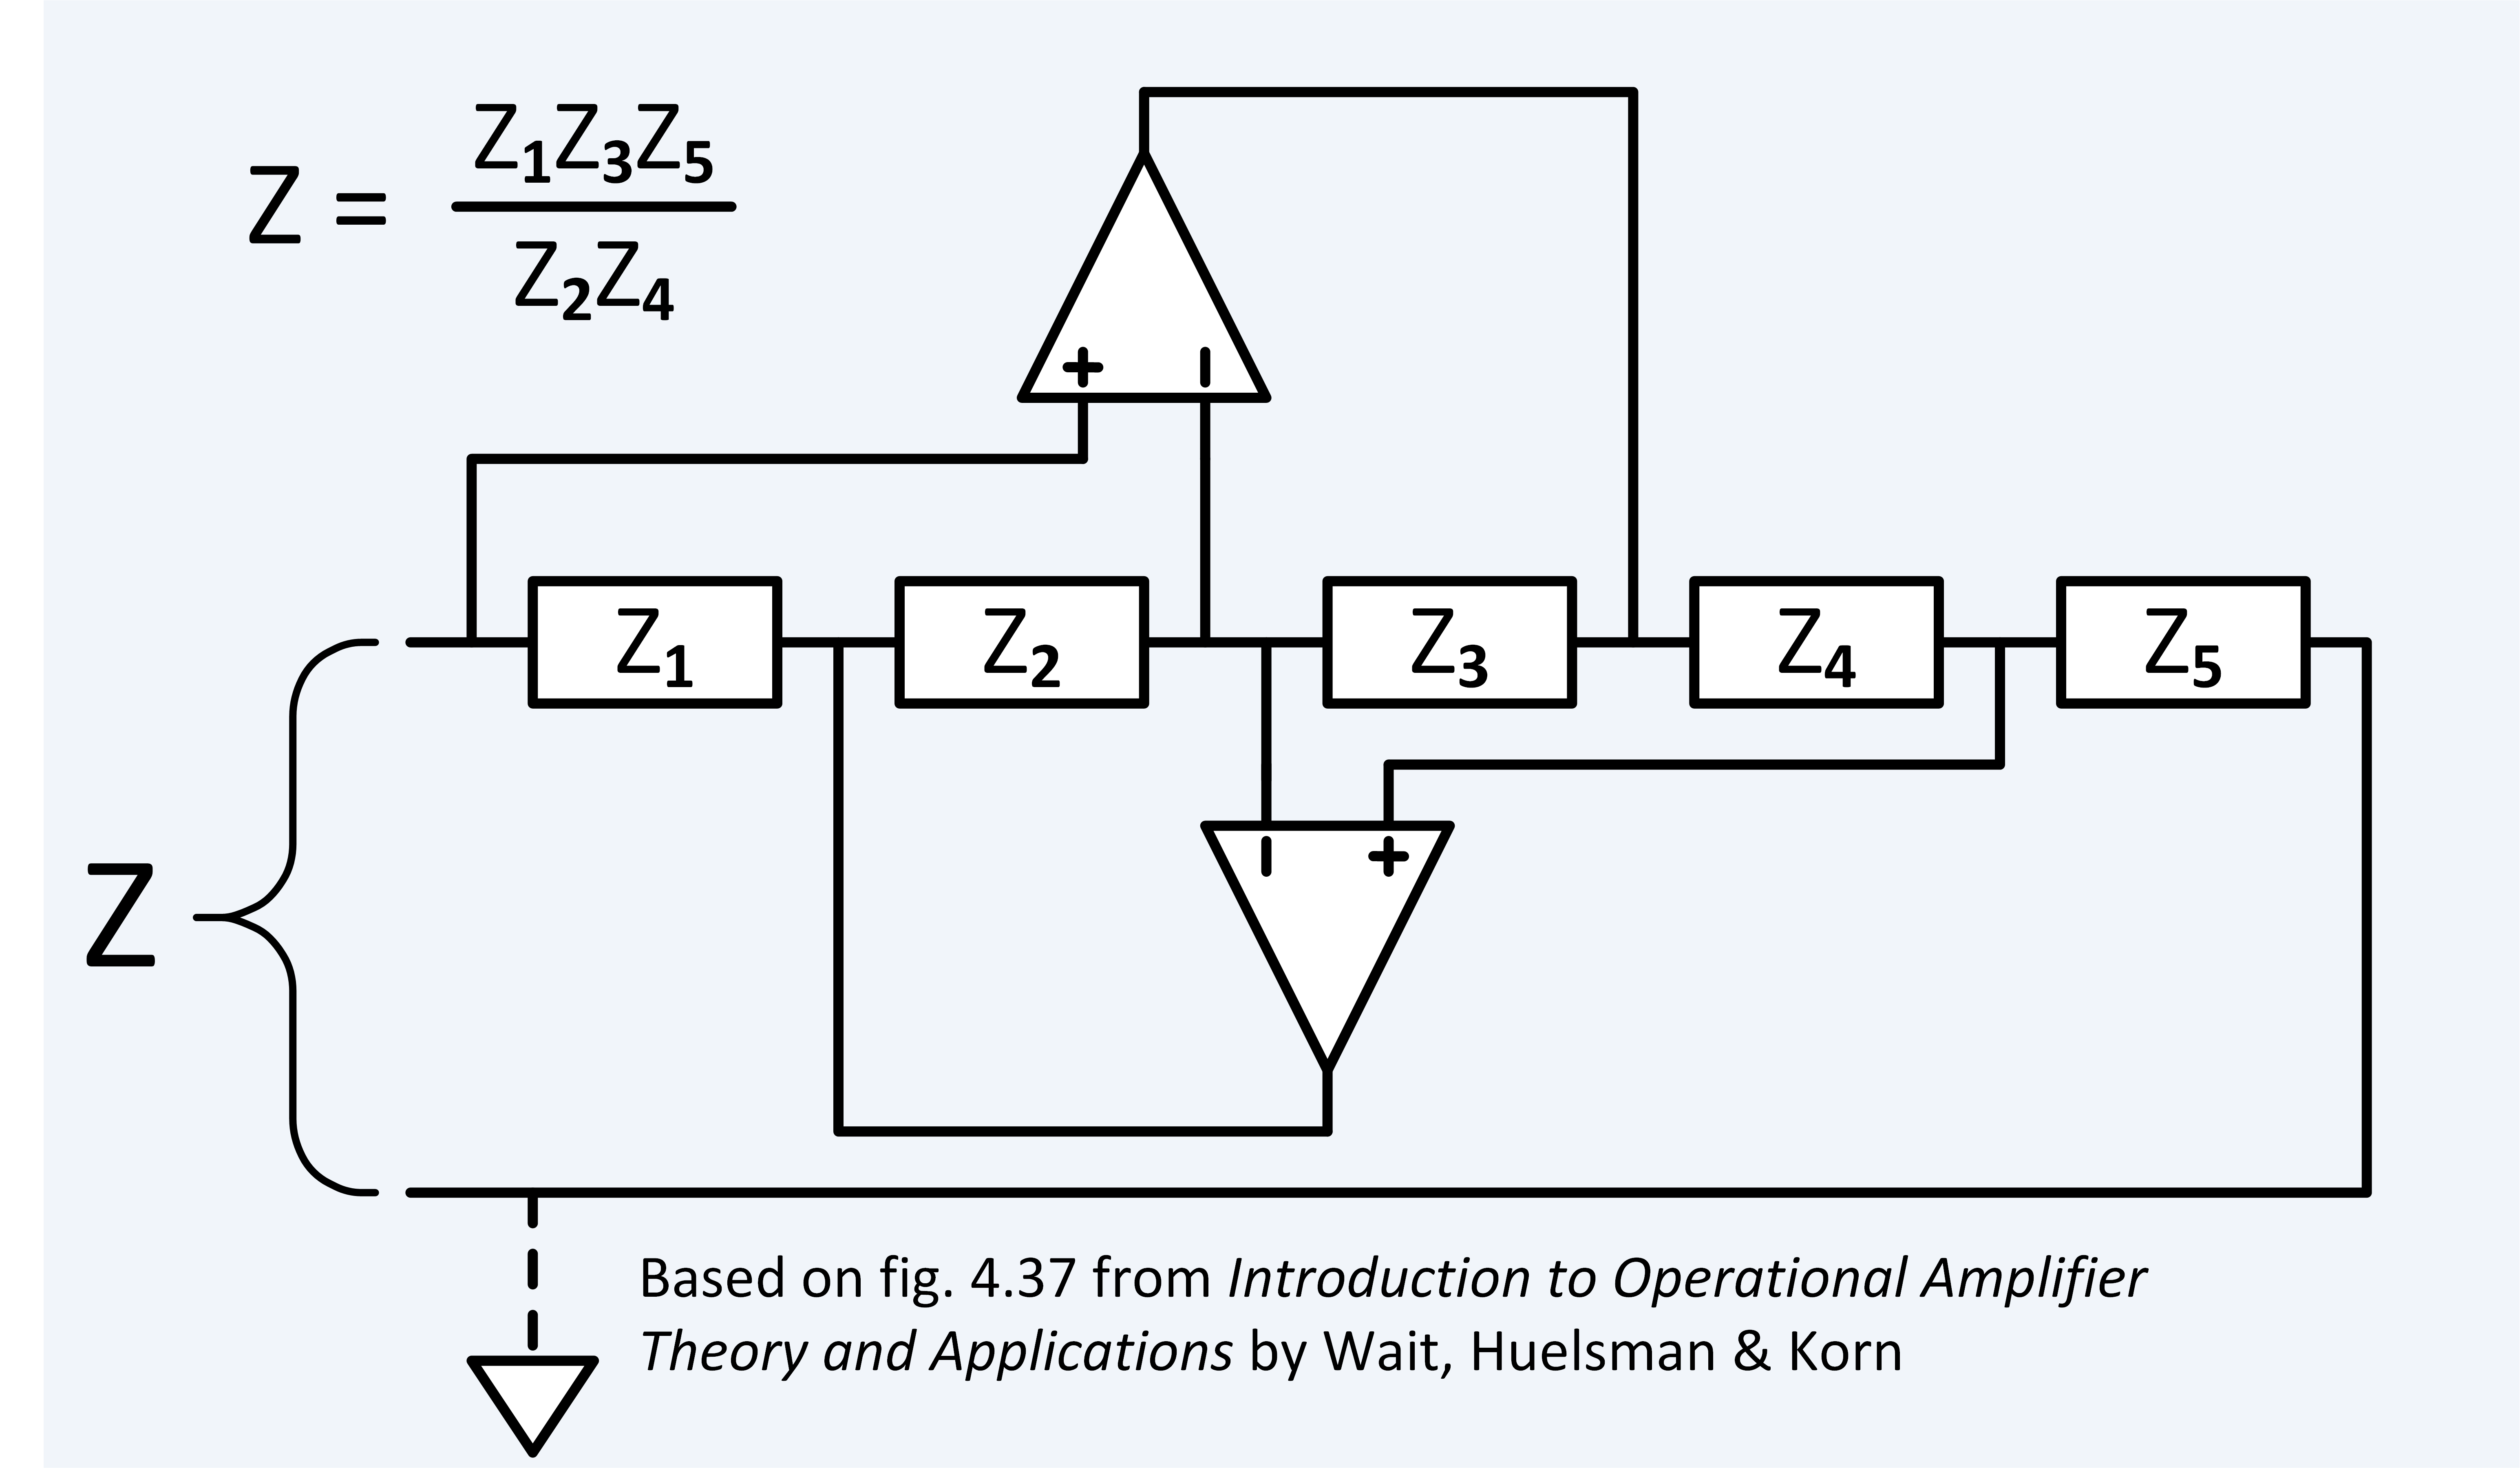
\includegraphics[width=\linewidth]{./FIG/GIC.png}
    \caption{Generalized Impedance Converter (GIC)}
\end{figure}

\begin{equation}
    Z=Z_{in}=\frac{Z_1Z_3Z_5}{Z_2Z_4}
\end{equation}




\subsection{Simulated Inductors}
In this method of designing Higher order active filter, we use simulated inductors to simulate thr grounded inductor in a passive circuit. In the above figure if value of all impedance except $Z_5$  is 1 i.e $Z_1=Z_2=Z_3=1 \Omega, Z_4= 1 F$ and $Z_5=k\Omega$. Then new value of $Z$ will be
\begin{equation*}
    Z=Z_{Simulated Inductor}=\ddfrac{1\times1\times k}{\left(\frac{1}{s}\right)\times1}=ks
\end{equation*}



\subsection{Frequency Dependent Negative Resistor (FDNR)}
Burton’s FDNR technique involves eliminating the use of inductor by scaling all impedances by frequency dependent factor $\frac{1}{s}$ converting a resistor to a capacitor $\left(\ddfrac{R}{s}\right)$, an inductor to a resistor $(L)$, and the capacitor to a Frequency Dependent Negative Resistor (FDNR) $\left(\ddfrac{1}{s^2C}\right)$ with symbol  $\|\|$ .
In the above figure if $Z_1=Z_2=1$ $\Omega$, $Z_3=Z_5=1$ F and $Z_4=k$ $\Omega$ is used. Then new value of $Z$ will be
\begin{equation*}
    Z=Z_{FDNR}=\ddfrac{\left(\frac{1}{s}\right)\times\left(\frac{1}{s}\right)\times 1}{1\times k}=\frac{1}{ks^2}
\end{equation*}

\subsection{Leapfrog Simulation}
This method simulates the operation of the ladder rather than its components by modeling all circuit equations and the voltage--current relationship of the elements.Simulation involve step of determining lowpass prototype, identifying admittance and impedance of the ladder, selecting Leapfrog parameters, and simulating the circuit.If needed frequency and Magnitude scaling is performed .




%%Exercises
\pagebreak
\section{Exercises:}

\begin{figure}[H]
    \centering
    \scalebox{1.25}
    \figquestion
    \caption{Fourth order Butterworth lowpass ladder circuit}
\end{figure}

%Question 1
\begin{Q}
    {
        The network given in figure 1 is the fourth order Butterworth lowpass filter at normalized
        frequency of 1 rad/sec. From this network, design a lowpass filter having half power frequency of
        20000 rad/sec using FDNR. Realize the network and observe the magnitude response.}
\end{Q}
After applying Bruton's Transformation on above circuit we get,

\begin{figure}[H]
    \centering
    \scalebox{1.25}
    \figfdnr
    \caption{Fourth order Butterworth Lowpass Circuit using FDNR}
\end{figure}

Using magnitude scaling factor of $K_m=\ddfrac{1}{s}$ on Figure 2, we get,
\begin{equation*}
    \begin{aligned}
         & Z'_{R\textsubscript{$1$}}=1 \text{ F} \quad           &  & Z'_{R\textsubscript{$2$}}=1 \text{ F}           \\
         & Z'_{L\textsubscript{$1$}}=0.7654 \text{ }\Omega \quad &  & Z'_{L\textsubscript{$2$}}=1.848 \text{ }\Omega  \\
         & \text{(FDNR)  } Z'_{C\textsubscript{$1$}}=1.848 \quad &  & \text{(FDNR)  }Z'_{C\textsubscript{$2$}}=0.7654 \\
    \end{aligned}
\end{equation*}

To realize first FDNR $Z'_{C\textsubscript{$1$}}$ we use  $Z_1=Z_2=1$ $\Omega$, $Z_3=Z_5=1$ F and $Z_4=k$ $\Omega$,
\begin{equation*}
    \begin{aligned}
        Z_{in} & =Z'_{C\textsubscript{$1$}}=\ddfrac{1\times\left(\frac{1}{s}\right)\times\left(\frac{1}{s}\right)}{1\times k} \\
               & \frac{1}{1.848s^2}=\frac{1}{ks^2}                                                                            \\
               & \therefore k=1.848 \text{ }\Omega
    \end{aligned}
\end{equation*}
To realize Second FDNR $Z'_{C\textsubscript{$2$}}$ we use  $Z_1=Z_2=1$ $\Omega$, $Z_3=Z_5=1$ F and $Z_4=k$ $\Omega$,
\begin{equation*}
    \begin{aligned}
        Z_{in} & =Z'_{C\textsubscript{$2$}}= \frac{1}{0.7654s^2}=\frac{1}{ks^2} \\
               & \therefore k=0.7654 \text{ }\Omega
    \end{aligned}
\end{equation*}

As per the question we require a halfpower frequency of 20000 rad/sec so, Frequency Scaling is calculated to $K_f$=2000.

Thus final value will be after Frequency scaling $K_f=20000 $  and Impedance Scaling $K_m=1000$.

\begin{table}[H]
    \centering
    \begin{tabular}[H]{| m{10em}|m{10em}|m{14em}|}
        \hline
        \rowcolor[rgb]{0.569,0.647,0.947}
        \textbf{Component Symbol}
                                    & \textbf{Normalized value }
                                    & \textbf{Final value after scaling}                   \\
        \hline
        $Z'_{R\textsubscript{$1$}}$ & 1 $F$                              & 50$nF$          \\ \hline
        $Z'_{R\textsubscript{$2$}}$ & 1 $F$                              & 50$nF$          \\ \hline
        $Z'_{L\textsubscript{$1$}}$ & 0.7654$\Omega$                     & 765 $\Omega$    \\ \hline
        $Z'_{L\textsubscript{$1$}}$ & 1.848 $\Omega$                     & 1.848 $K\Omega$ \\ \hline
    \end{tabular}
    \caption{Component Values of LPF excluding FDNR's}
\end{table}

\begin{table}[H]
    \centering
    \begin{tabular}[H]{| m{10em}|m{10em}|m{14em}|}
        \hline
        \rowcolor[rgb]{0.569,0.647,0.947}
        \textbf{Component Symbol}
              & \textbf{Normalized value }
              & \textbf{Final value after scaling}                   \\
        \hline
        $Z_1$ & 1 $\Omega$                         & 1$K\Omega$      \\ \hline
        $Z_2$ & 1  $\Omega$                        & 1$K\Omega$      \\ \hline
        $Z_3$ & 1$F$                               & 50 $nF$         \\ \hline
        $Z_4$ & 1.848 $\Omega$                     & 1.848 $K\Omega$ \\ \hline
        $Z_5$ & 1 $F$                              & 50$nF$          \\ \hline
    \end{tabular}
    \caption{Component Values of First FDNR  $Z'_{C\textsubscript{$1$}}$}
\end{table}

\begin{table}[H]
    \centering
    \begin{tabular}[H]{| m{10em}|m{10em}|m{14em}|}
        \hline
        \rowcolor[rgb]{0.569,0.647,0.947}
        \textbf{Component Symbol}
              & \textbf{Normalized value }
              & \textbf{Final value after scaling}                 \\
        \hline
        $Z_1$ & 1 $\Omega$                         & 1$K\Omega$    \\ \hline
        $Z_2$ & 1  $\Omega$                        & 1$K\Omega$    \\ \hline
        $Z_3$ & 1$F$                               & 50 $nF$       \\ \hline
        $Z_4$ & 0.7654 $\Omega$                    & 765 $K\Omega$ \\ \hline
        $Z_5$ & 1 $F$                              & 50$nF$        \\ \hline
    \end{tabular}
    \caption{Component Values of Second FDNR  $Z'_{C\textsubscript{$2$}}$}
\end{table}

\Porcirobs{0.95}{low pass FDNR}{-6.02}{3.1765}


\pagebreak
%Question 2
\begin{Q}
    {Obtain a Highpass filter at normalized frequency of 1 rad/sec from the lowpass filter given in
        figure 1 using frequency transformation. From the circuit obtained, design a Highpass filter using simulated inductors. In your final design the half power frequency should be 4775 Hz and practically realizable elements. Realize the filter network. Also observe and analyze the magnitude response of the filter network.}
\end{Q}

Applying frequency transformation to get Highpass filter at normalized frequency of 1 rad/sec, we get,
\begin{figure}[H]
    \centering
    \scalebox{1.25}
    \fighp
    \caption{Fourth order Highpass ladder circuit at at normalized frequency of 1 rad/sec}
\end{figure}

To realize the inductor $Z'_{C\textsubscript{$1$}}$ we use  $Z_1=Z_2=Z_3=1$ $\Omega$, $Z_4=1$ F and $Z_5=k$ $\Omega$, we get,
\begin{equation*}
    \begin{aligned}
        Z_{in} & =Z'_{C\textsubscript{$1$}}=\ddfrac{1\times1\times k}{\left(\frac{1}{s}\right)\times 1} \\
               & \Rightarrow 0.5411s=s\times k                                                          \\
               & \therefore k=0.5411 \text{ }\Omega
    \end{aligned}
\end{equation*}


Similarly, for the inductor $Z'_{C\textsubscript{$1$}}=1.3605 \Omega$ we get $K=Z_5=1.3605 \Omega$.As we require the highpass filter having frequency of $4775$ Hz, a frequency scaling factor of $K_f=\ddfrac{2\pi\times4775}{1}\approx 3*10^4$ is used and  a magnitude scaling factor of $K_m=10^3$ is used. Hence a final value obtained will be after Frequency and Magnitude scaling,


\begin{table}[H]
    \centering
    \begin{tabular}[H]{| m{10em}|m{10em}|m{14em}|}
        \hline
        \rowcolor[rgb]{0.569,0.647,0.947}
        \textbf{Component Symbol}
                                    & \textbf{Normalized value }
                                    & \textbf{Final value after scaling}               \\
        \hline
        $Z'_{R\textsubscript{$1$}}$ & 1 $\Omega$                         & 1 $K\Omega$ \\ \hline
        $Z'_{R\textsubscript{$2$}}$ & 1 $\Omega$                         & 1 $K\Omega$ \\ \hline
        $Z'_{L\textsubscript{$1$}}$ & 0.1.3065 $F$                       & 45.35 $nF$  \\ \hline
        $Z'_{L\textsubscript{$1$}}$ & 0.5411 $F$                         & 18.04 $nF$  \\ \hline
    \end{tabular}
    \caption{Component Values of HPF excluding FDNR's}
\end{table}

\begin{table}[H]
    \centering
    \begin{tabular}[H]{| m{10em}|m{10em}|m{14em}|}
        \hline
        \rowcolor[rgb]{0.569,0.647,0.947}
        \textbf{Component Symbol}
              & \textbf{Normalized value }
              & \textbf{Final value after scaling}                \\
        \hline
        $Z_1$ & 1 $\Omega$                         & 1$K\Omega$   \\ \hline
        $Z_2$ & 1  $\Omega$                        & 1$K\Omega$   \\ \hline
        $Z_3$ & 1 $\Omega$                         & 1$K\Omega$   \\ \hline
        $Z_4$ & 1 $F$                              & 33.33 $nF$   \\ \hline
        $Z_5$ & 0.5411 $\Omega$                    & 541 $\Omega$ \\ \hline
    \end{tabular}
    \caption{Component Values of simulated inductor  $Z'_{C\textsubscript{$1$}}$}
\end{table}

\begin{table}[H]
    \centering
    \begin{tabular}[H]{| m{10em}|m{10em}|m{14em}|}
        \hline
        \rowcolor[rgb]{0.569,0.647,0.947}
        \textbf{Component Symbol}
              & \textbf{Normalized value }
              & \textbf{Final value after scaling}                  \\
        \hline
        $Z_1$ & 1 $\Omega$                         & 1$K\Omega$     \\ \hline
        $Z_2$ & 1  $\Omega$                        & 1$K\Omega$     \\ \hline
        $Z_3$ & 1 $\Omega$                         & 1$K\Omega$     \\ \hline
        $Z_4$ & 1 $F$                              & 33.33 $nF$     \\ \hline
        $Z_5$ & 1.3605 $\Omega$                    & 1.36 $K\Omega$ \\ \hline
    \end{tabular}
    \caption{Component Values of simulated inductor  $Z'_{C\textsubscript{$2$}}$}
\end{table}

\Porcirobs{0.95}{high pass simulated inductor}{-6.02}{4.857}




\pagebreak


%Question 3
\begin{Q}
    {From the circuit given in figure 1, design a lowpass passive filter having half power frequency of
        40000 rad/sec with practically suitable elements, using Leapfrog simulation. Realize the filter
        network and observe the magnitude response of the network.}
\end{Q}


We can represent the figure 2 as,
\begin{figure}[H]
    \centering
    \scalebox{1.5}
    \figleap
    \caption{Block diagram representation of the fourth order Butterworth lowpass filter}
\end{figure}

Applying voltage and nodal analysis for Figure 9 , we get,
\begin{equation*}
    \begin{aligned}
         & I_1=\frac{V_1-V_3}{Z_1}=T_1(V_1-V_3)  \\
         & V_3=Z_2(I_1-I_2)=T_2(I_1-I_2)         \\
         & I_2=\frac{V_3-V_4}{Z_3}= T_3(V_3-V_4) \\
         & V_4=Z_4I_2=T_4I_2
    \end{aligned}
\end{equation*}


Where,
\begin{equation*}
    \begin{aligned}
         & T_1=\frac{1}{Z_1}=\frac{1}{1+0.7654s} \\
         & T_2=Z_2=\frac{1}{1.848s}              \\
         & T_3=\frac{1}{Z_3}=\frac{1}{1.848s}    \\
         & T_4=Z_4=\frac{1}{1+0.7654s}
    \end{aligned}
\end{equation*}

Let $V_{I1}=I_1$ and $V_{I2}=I_2$ and rearranging the signs we get,
\begin{equation}
    V_{I1}=-(-T_1)(V_1-V_3)
\end{equation}
\begin{equation}
    -V_3=-T_2(V_{I1}-V_{I2})
\end{equation}
\begin{equation}
    -V_{I2}=-(-T_3)(V_4-V_3)
\end{equation}
\begin{equation}
    V_4=(-T_4)(-V_{I2})
\end{equation}

Above equation can be represented in block Diagram as,
\begin{figure}[H]
    \centering
    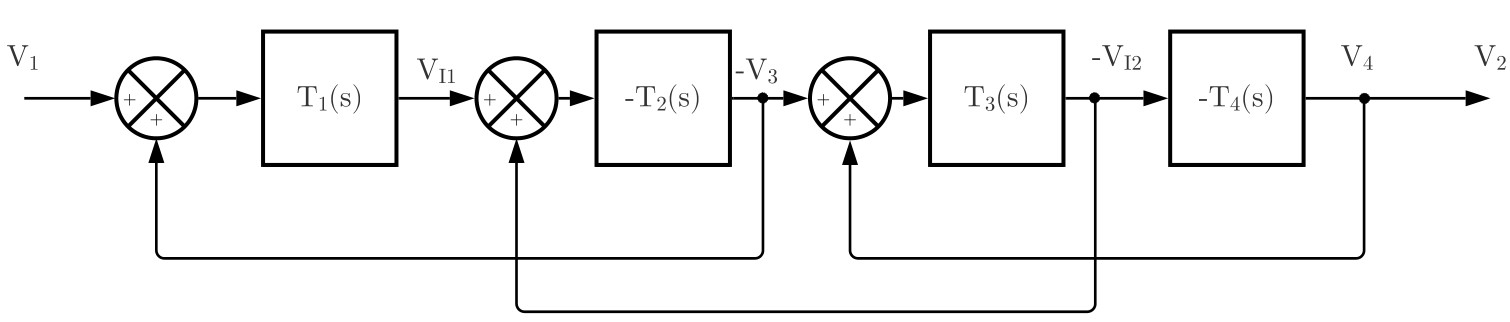
\includegraphics[width=\linewidth]{./FIG/Block rep.jpg}
    \caption{Block diagram representation of circuit equations}
\end{figure}


\begin{figure}[H] %%%%%%%%%%%proteus circuit
    \centering
    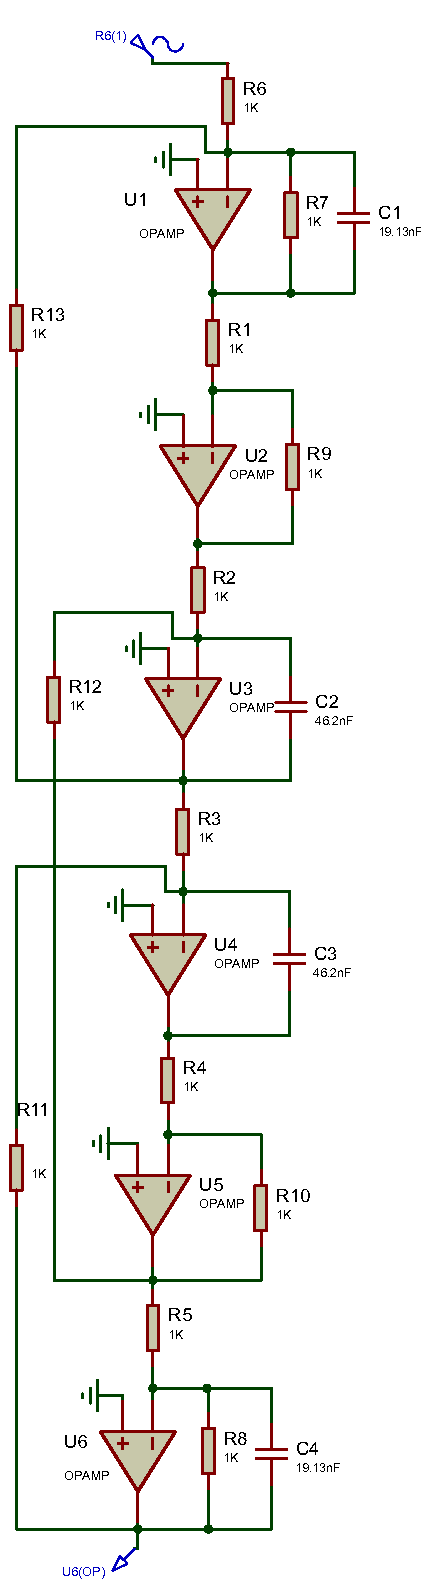
\includegraphics[width=0.39\linewidth]{./FIG/P_cir_figlow pass leapfrog.PDF}
    \caption{Proteus Circuit for low pass Leapfrog}
\end{figure}

\Pobs{0.95}{low pass leapfrog}{0}{4.807}


%section for Discussion and Conclustion
\section{Discussion and Conclusion}
In this lab we designed the higher order filter using Active simulation of passive circuit. We used simulated inductors, FDNR and Leapfrog Simulation to design the filter. GIC is extensively used in above discussed methods.
We also simulated the circuits designed using these methods and observe its magnitude hence fulfilling our Lab objective.



\end{document}